\documentclass[12pt]{article}

\usepackage[letterpaper, margin=1in]{geometry} % get the page set up correctly
\pagenumbering{gobble}
\usepackage{amsmath,amssymb} % math symbols
\usepackage[section]{placeins} % put the floats in the section they come from always
\usepackage{authblk} % authors
\usepackage{siunitx} % SI units
\usepackage{graphicx} % to include graphics
\usepackage{natbib} % references
\usepackage{physics} % math notation and vectors
\usepackage{wrapfig}

\usepackage{tikz}
\usetikzlibrary{
	shapes,
    arrows,
    shapes.geometric,
    positioning,
}

% Define block styles
\tikzstyle{object} = [
	rectangle,
    draw,
    fill=blue!40,
    text width=9cm,
    text badly centered,
    rounded corners]

\tikzstyle{action} = [
	rectangle,
	draw,
    text width=9cm,
    text centered,
    rounded corners]

\tikzstyle{arrow} = [draw, -latex']
\tikzstyle{noarrow} = [draw, dashed]

% set consistent font size
\tikzset{every picture/.style={font issue=\footnotesize},
         font issue/.style={execute at begin picture={#1\selectfont}}
         }


% code input
\renewcommand{\scriptsize}{\fontsize{8pt}{8pt}\selectfont}
\usepackage{listings,float}
\newfloat{lstfloat}{htbp}{lop}
\floatname{lstfloat}{Listing}
\lstset{
    language=R,
    basicstyle=\scriptsize\ttfamily,
    stepnumber=1,
    numbersep=3pt,
    showspaces=false,
    showstringspaces=false,
    showtabs=false,
    frame=single,
    tabsize=2,
    captionpos=b,
    breaklines=true,
    breakatwhitespace=false,
    escapeinside={},
    keywordstyle={},
    morekeywords={}
}

% These calls come last
\usepackage[hidelinks]{hyperref} % to simplify the use of \href
\usepackage{cleveref} % better cross-references


\bibliographystyle{agu}
\graphicspath{{../figs/}}

\title{Global-Local Interactions Modulate Tropical Moisture Export to the Ohio River Basin}
\author[1,2]{James Doss-Gollin}
\author[1,2]{David Farnham}
\author[1,2]{Upmanu Lall}
\affil[1]{Columbia Water Center}
\affil[2]{Department of Earth and Environmental Engineering, Columbia University}

\date{\today}

\begin{document}

\def\ci{\perp\!\!\!\perp}
\def\ex{\mathbb{E}}
\def\prob{\mathbb{P}}
\def\ind{\mathbb{I}}
\def\grad{\triangledown}
\def\bigo{\mathcal{O}}
\def\normal{\mathcal{N}}
\def\bern{\text{Bernoulli}}
\def\logit{\text{logit}}
\def\binom{\text{Bin}}
\def\poiss{\text{Poiss}}
\def\cauchy{\text{Cauchy}}
\def\sigmoid{\vb{\sigma}}
\def\given{\big|}
\def\stan{\texttt{Stan~}}
\maketitle
%%%%%%%%%%%%%%%%%%%%



\section{Conceptual Framework}

Managing and adapting flood risk requires estimates of the joint distribution of flood frequency and intensity into the future.
While traditional approaches have taken either purely statistical or model chaining (climate model to hydrological model) paths, we view floods as being caused by a \emph{hierarchy of causal mechanisms} \cite[see][]{Merz2014}.
Specifically, we hypothesize that there is a unique set of atmospheric circulation mechanisms that can lead to sufficient large-scale transport and convergence of moisture for extreme regional flooding.
By identifying these circulation mechanisms and exploring their conditional probabilities given relatively lower-frequency and more predictable atmospheric circulation states, we hope to improve the ability to simulate extreme rainfall conditionally from forecasts.
Ultimately, this will allow us to \emph{simulate the quantity of interest conditionally on forecast or hypothesized low-frequency variables}.



\citet{Lavers2016} show that extreme moisture flux is more predictable than extreme rainfall on the West Coast, and for this reason we use integrated water vapor transport into the Ohio River Basin

\begin{figure}
    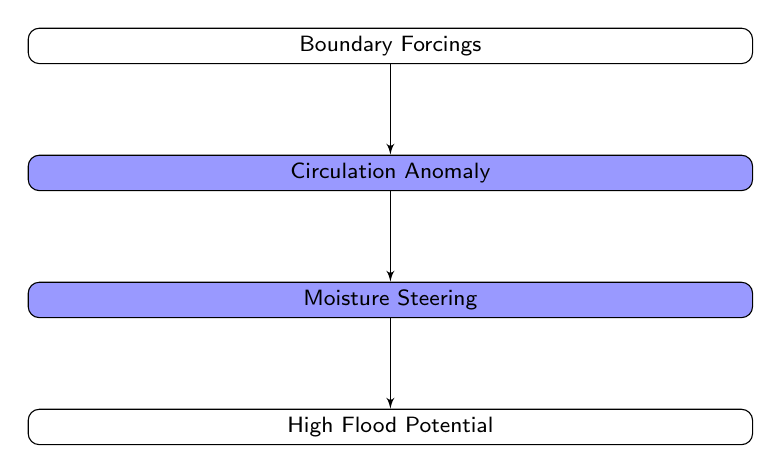
\begin{tikzpicture}[node distance = 1.15cm, auto, font=\sffamily]
	% Place nodes
	\node [action] (boundary) {Boundary Forcings};
	\node [object, below= of boundary] (circulation) {Circulation Anomaly};
	\node [object, below=of circulation] (steering) {Moisture Steering};
	\node [action, below= of steering] (flood) {High Flood Potential};
	% Draw edges
	\path [arrow] (boundary) -- (circulation);
    \path [arrow] (circulation) -- (steering);
    \path [arrow] (steering) -- (flood);
\end{tikzpicture}
~\hfill
    \includegraphics[width=0.6\textwidth]{flooding_2011_flooding}
    \caption{(L) Causal hierarchy for extreme, regional floods. (R) Tracked cyclones (lines) and monthly-mean \SI{250}{\hecto\pascal} winds for April 2011, coinciding with severe flooding in the Ohio and Upper Mississippi River Basins.}
    \label{fig:apr2011}
\end{figure}

\begin{figure}
    \centering
    \includegraphics[width=0.6\textwidth]{map_inset}
    \caption{A map of our study area. Shaded area is the Ohio River Basin, while the box denotes the area over which integrated water vapor transport is summed. Inset shows Eastern United States with Ohio River Basin in blue.}
    \label{fig:study-area}
\end{figure}
\begin{figure}
    %\includegraphics{/path/to/figure}
    \caption{\texttt{Would be great to add here a conceptual diagram}}
    %\label{}
\end{figure}


\section{Exploratory Findings}

\subsection{Preferred Cyclone Pathway Associated with High Moisture Flux}

To associate cyclone tracks with the observed moisture flux, I simply associate each 6-hour track position with the concurrent moisture transport into the black box shown in \cref{fig:study-area}.
\Cref{fig:position-given-flux} shows the moisture flux associated with these cyclones within a \SI{25}{\degree} radius of the black box.
The most apparent feature is a region directly to the North-West of the Ohio River Basin where cyclone occurrence signifies a very high expected moisture flux.
In this region, the flux is high relative to the climatological moisture flux shown in \cref{fig:flux-distribution}.
\begin{figure}
    \centering
    \includegraphics[width=0.5\textwidth]{moisture_cyclone_q_distribution}
    \caption{Climatological DJF Moisture flux distribution into the Ohio River basin}
    \label{fig:flux-distribution}
\end{figure}
\begin{figure}
    \centering
    \includegraphics[width=0.75\textwidth]{moisture_cyclone_dq_given_locn}
    \caption{Cyclone locations and associated moisture flux. Color indicates net moisture flux into the black box, in $\SI{1e4}{\kilo\gram\per\meter\per\second}$. }
    \label{fig:position-given-flux}
\end{figure}

It is also useful to associate moisture flux with full cyclone tracks, rather than their instantaneous locations.
To do this I take the maximum instantaneous flux experienced along the track of the cyclone\footnote{this leaves a lot to be desired -- suggestions welcome} for each track.
\Cref{fig:tracks-given-flux} shows the tracks that led to extreme (97.5 quantile exceedance) moisture flux versus a bootstrap of all cyclones.
A clear preferred pathway is apparent for the cyclone tracks that are associated with high moisture flux.
\begin{figure}
    \centering
    \includegraphics[width=0.8\textwidth]{moisture_cyclone_tracks_given_flux}
    \caption{(R) Cyclone tracks associated with high moisture flux; (L) a bootstrap sample, of equal size, of randomly chosen cyclone tracks. Cyclone intensity computed following \citet{Booth2015} and rescaled as $\log \qty(-I)$.}
    \label{fig:tracks-given-flux}
\end{figure}

This is consistent with our previous findings looking at extreme rainfall in the region, where we have found that extreme rainfall in this region is associated with a ridge to the East (often persistent), and a transient low pressure whose exact location varies but generally leads to a dipole (or, looking farther to the West, a tripole) patter.
We have found that this leads to the expected anomalous moisture transport, again consistent with previous findings from our own work and others \citep{Nakamura2012,Lavers2013a,Steinschneider2016a}.


\subsection{PNA Influence}

There is a well-documented \citep[ie][]{Nakamura2012,Robertson2015,Steinschneider2015a} link between the PNA oscillation and extreme rainfall or flooding in this region.
\Cref{fig:tracks-given-pna} shows cyclone tracks associated with negative, neutral, and positive phases of the PNA (only Eastern North America is shown).
The pathway associated with intense moisture vapor transport shown in \cref{fig:tracks-given-flux} is clearly enhanced during the negative PNA phase, and suppressed during the positive phase.
Preliminary further analysis suggests that this may be due to both steering and to the ehnahcement/suppression of cyclogenesis in particular regions that tend to track to/away from this high-moisture path.\footnote{If you know more about this, I'd be interested to learn more}

\begin{figure}
    \centering
    \includegraphics[width=0.8\textwidth]{pna_cyclone_map_plot}
    \caption{Cyclone tracks associated with the (L) negative, (C) neutral, and (R) positive terciles of the daily PNA index.  Cyclone intensity as \cref{fig:tracks-given-flux}.}
    \label{fig:tracks-given-pna}
\end{figure}

\section{Data Used}

I use ERA-Interim reanalysis \citep{Dee2011}.
The cyclone tracks are courtesy of Donna Lee who generated them from ERA-Interim sea level pressure using the methodology of \citet{Hodges1994} and whose results have been verified in \cite{Booth2015}.
The PNA and AMO data from from the NCEP web site.

\section{Statistical Modeling}


\subsection{Variable Summary} \label{sec:var-summary}


The variables I include in my analysis are the following
\begin{description}
    \item[Moisture Flux] the summed moisture flux into the black box in \cref{fig:study-area}. Units are in \SI{10000}{\kilo\gram H_2O \per\meter\per\second}
    \item[SSTs] Mean sea surface temperature over a box covering the Gulf of Mexico. Units are in \si{\kelvin} and have been rescaled to the standard normal.
    \item[Dipole low] The geopotential height anomaly over the Eastern North America box defined in \citet{Farnham2016}. Units are in \si{\pascal} and have been rescaled to the standard normal.
    \item[Dipole high] The geopotential height anomaly over the Western North Atlantic box defined in \citet{Farnham2016}. Units are in \si{\pascal} and have been rescaled to the standard normal.
    \item[PNA] daily PNA index. Units are standardized for all seasons; the DJF distribution is not fully a standard normal.
    \item[AMO] monthly AMO index. Units are standardized for all seasons; the DJF distribution is not fully a standard normal.
    \item[weight] See \cref{sec:challenges}
\end{description}
\Cref{sec:parameters} showx the joint and marginal distributions of these parameters.

\subsection{Model Implementation}

The \stan code for my model implementation is shown in \cref{sec:stan}.
This model takes requires three fundamental data blocks:
\begin{enumerate}
    \item $y_{N \times 1}$, the observed data (in this case, the moisture flux)
    \item $X_{N \times p}$, the ``local'' factors that directly govern the $y$
    \item $Z_{N \times k}$, the ``global'' factors that are hypothesized to govern the $X$
\end{enumerate}
then, the model is formulated
\begin{align}
    y_t & \sim \normal \qty(\beta_0 + X'_t \beta, \sigma^2) \quad t = 1, \ldots, T \label{eq:yX}\\
    X_{t,j} &\sim \normal \qty(\alpha_{0,j} + Z'_t \alpha_j, \tau_j^2) \quad j = 1, \ldots, p \label{eq:XZ}
\end{align}
$\normal$ signifies the univariate normal distribution.
An example of this is implemented below.
The coefficients are somewhat hard to interpret; in this example, $X$ contains first the 0-1 cyclone hit score and second the value of the high box of the dipole from our previous paper.
$Z$ contains the daily PNA index.

\subsection{Results}

The posterior
\begin{lstfloat}
    \lstinputlisting{../bayesian/stan_out.txt}
    \caption{Summary of posterior distributions estimated in \stan  \label{stan:fit}}
\end{lstfloat}
\begin{figure}
    \centering
    \includegraphics[width=\textwidth]{bayesian_posterior}
    \caption{Posterior parameter distributions}
    \label{label:stan-plot}
\end{figure}


This inference, summarized in Listing \ref{stan:fit}, are slightly difficult to interpret.
\Cref{sec:var-summary} shows the actual units of the physical quantities.

Examining the $\beta_1,\beta_2$ values, we see that increasing the amplitude of the eastern ridge by one standard deviation produces approximately the same impact (slightly higher) as a cyclone `hit' on moisture flux, but that both lead to large increases in expected moisture flux.
Exploring the second-order ($X$ dependence on $Z$) effects (note that the $X$ have different units here), we see that increasing the Gulf of Mexico SSTs, a positive AMO, and a negative PNA all lead to an expected increase in the Western Atlantic Ridge anomaly.
However, the impacts of the AMO and Gulf of Mexico SSTs on the probability of a cyclone hit are relatively small, though a negative PNA increases the probability.

These findings are in line with expectation from first principles and previous observational studies, but have not (to my knowledge) been simulatneously estimated in a Bayesian context.
They are also in line with the statistical hypothesis that \emph{all} the interactions have some \emph{non-zero} effect, but that a small subset of effects are large.
Thus, hypothesis testing against a null hypothesis that the effect magnitude is exactly zero is not meaningful for describing effect sizes.

While it is not a full posterior model check, it is helpful to examine the simulation traces of the simulation to ensure model mixing and convergence.
\Cref{label:stan-trace} shows that convergence and mixing is excellent for all parameters observed.
\begin{figure}
    \centering
    \includegraphics[width=\textwidth]{bayesian_traceplot}
    \caption{Traceplot of posterior simulations}
    \label{label:stan-trace}
\end{figure}


\section{Ongoing Challenges} \label{sec:challenges}

The first challenge I see is to identify intelligent and robust priors for the model specified in \cref{eq:yX,eq:XZ}.
I'm interested in potentially using Cauchy parameters to encourage sparsity but haven't yet tested this.

I also need a way to parameterize the cyclone location.
Ideally I'd like to come up with a one-dimensional index (though 2-D would be OK) that could score whether there is a cyclone track centered in a region of interest.
\Cref{fig:position-given-flux} shows that there is a clear relationship between the locations of extratropical cyclones and moisture transport into the Ohio River Basin.
In particular, there is a South-East to North-West pattern where tracks associated with high moisture flux are associated.
I'm currently parameterizing this as a zero-one hit score over a parallelogram that roughly captures this area, but I'd like to do better.

Finally, I need to add more parameters to the model and perform model checking; my linear normal assumptions may not make very much sense.



%%%%%%%%%%%%%%%%%%%%

\clearpage
\bibliography{../library.bib}

\clearpage
\appendix
\section{Stan Code} \label{sec:stan}
\lstinputlisting{../bayesian/Model1.stan}

\section{Joint and Marginal Distributions} \label{sec:parameters}
\begin{figure}
    \centering
    \includegraphics[width=0.8\textwidth]{joint_distribution_everything}
    \caption{The pairwise distributions of the model parameters}
    \label{fig:joint-distributions}
\end{figure}
\begin{figure}
    \centering
    \includegraphics[width=0.8\textwidth]{marginal_distributions}
    \caption{The marginal distributions of the model parameters}
    \label{fig:joint-distributions}
\end{figure}

\end{document}
